\documentclass[a4paper,12pt]{report}

% --- PREAMBOLO ---
\usepackage[a4paper]{geometry}
\usepackage{amssymb,amsmath,amsthm}
\usepackage{graphicx}
\usepackage{url}
\usepackage{epsfig}
\usepackage[italian]{babel}
\usepackage{setspace}
\usepackage{tesi} 
\usepackage{wrapfig}
\usepackage[hidelinks]{hyperref}
\usepackage[export]{adjustbox}
\usepackage{epigraph}
\usepackage{blindtext}
\usepackage{subfig} % per le figure con più pannelli (a, b, c)
\usepackage{booktabs} % per le tabelle formattate correttamente (senza linee verticali) 

\usepackage[utf8]{inputenc}
\usepackage[disable]{todonotes} %per note e commenti
%quando mando bozza -> \usepackage[disable]{todonotes}

\usepackage{csquotes}
% --- BIBLIOGRAFIA: motore biblatex/biber per citazioni a piè di pagina ---
\usepackage[backend=biber, citestyle=verbose-ibid, bibstyle=numeric, sorting=none]{biblatex}
\addbibresource{bibliografia.bib}

\newtheorem{myteor}{Teorema}[section]
\newenvironment{teor}{\begin{myteor}\sl}{\end{myteor}}

% --- NUMERAZIONE CAPITOLI IN LETTERE (richiesta Prof. Buffa: "Capitolo Primo", non "Capitolo 1") ---
\usepackage{titlesec}

% Creiamo un convertitore invisibile per il titolo
\newcommand{\capitoloInLettere}{%
  \ifcase\value{chapter}\or Primo\or Secondo\or Terzo\or Quarto\or Quinto\or Sesto\or Settimo\or Ottavo\or Nono\or Decimo\fi
}

% Ridisegniamo la grafica del titolo della pagina
\titleformat{\chapter}[display]
  {\normalfont\huge\bfseries}
  {\chaptertitlename\ \capitoloInLettere} % Qui stampa la magia: "Capitolo Primo"
  {20pt}
  {\Huge}

% --- TITOLO E DATI ---
\begin{document}
\title{Sistemi d'Arma Autonomi Letali: \\criticità nel trattamento dei dati sensibili e analisi sperimentale tra vulnerabilità algoritmiche e giuridiche}
\author{Daniele Intra}
\dept{Corso di Laurea Magistrale in Sicurezza Informatica} 
\anno{2025-2026}
\matricola{53665A}
\relatore{Prof. Matteo Buffa}
\correlatore{Prof. Massimo Walter Rivolta}

% --- DEDICA E PREFAZIONE ---
\beforepreface

\prefacesection{Dedica}
{\hfill \Large {\sl Dedicato alle persone che amo, a tutti quelli che mi hanno affiancato in questo momento difficile della mia vita, alla mia famiglia, a mio nonno e mia nonna.
Dedicato a Manuel Pecchenini, che mi ha insegnato la forza di non arrendersi mai, a non mollare mai e a lottare per ciò in cui si crede.
Dedicato a chi lotta per un mondo più giusto e umano, ai milioni di bambini che soffrono ogni secondo in tutto il mondo, a chi non ha voce e a chi non ha diritto di parola.
Dedicato a tutte le studentesse e gli studenti che non sono piú qui con noi e che non hanno potuto scrivere una loro dedica, dedicato alla loro lotta contro un sistema scolastico e universitario che non li ha mai ascoltati e che li ha oppressi, rendendoli un corto ed invisibile servizio da telegiornale. 
Dedicato ai miei studenti, ex studenti, colleghi e alla Scuola, che mi ha permesso di crescere e di diventare la persona che sono oggi.
Dedicato a chi crede che la tecnologia possa essere un mezzo per il progresso e non una mera sostituzione di tutto quello che ci rende umani. }}

\prefacesection{Prefazione}
\begin{flushright}
\begin{minipage}{0.6\textwidth}
\epigraph{
    ``Il governo dei manganelli e dei plotoni di esecuzione, della carestia artificiale, dell'imprigionamento in massa e della deportazione di massa, non solo è inumano (nessuno se ne preoccupa più di tanto ai giorni nostri), ma è palesemente inefficiente, e in un'epoca di tecnologia avanzata l'inefficienza è un peccato mortale. Uno Stato totalitario davvero efficiente sarebbe quello in cui l'onnipotente potere esecutivo dei capi politici e il loro corpo manageriale controllano una popolazione di schiavi che non devono essere costretti ad esserlo con la forza perché amano la loro schiavitù.''
}{\textit{Aldous Huxley, Brave New World (1932)}}
\end{minipage}
\end{flushright}

Questo lavoro nasce da una profonda necessità di comprendere e resistere all'irrefrenabile insinuazione della \textit{techné} nella sfera più intima e vulnerabile dell'essere umano. In una società che chiede insistentemente di essere efficienti, produttivi, iperconnessi e miscelati con le macchine, è fondamentale interrogarsi sulle implicazioni sociali e politiche di questa trasformazione.
L'intelligenza artificiale in ambito militare ha infatti cessato di essere un semplice \textit{strumento} per diventare un vero e proprio \textit{agente}, spingendo il dibattito pubblico a concentrarsi quasi esclusivamente su dilemmi filosofici. Tuttavia, l'etica da sola si rivela inefficace se non viene tradotta in rigidi vincoli ingegneristici.
Rispetto a una canonica tesi in sicurezza informatica, questo lavoro si focalizza sulla dimensione umanitaria e giuridica per dimostrare una tesi ben precisa: la violazione dei diritti umani, nel contesto dei Sistemi d'Arma Autonomi Letali (LAWS), non deriva solo da ciniche scelte geopolitiche, ma anche e soprattutto da vulnerabilità architetturali intrinseche ai sistemi stessi. Criticità come i bias nei dati di addestramento, l'in-interpretabilità delle reti neurali (\textit{Black Box}), la suscettibilità al \textit{Data Poisoning} e agli \textit{Adversarial Attacks} si trasformano direttamente in danni collaterali sul campo.
Attraverso un'analisi interdisciplinare, la tesi si propone quindi di esplorare il trattamento dei dati sensibili e le fragilità algoritmiche dei LAWS, delineando come, in questo nuovo ecosistema bellico, la sicurezza informatica e la corretta architettura del software diventino il primo e ultimo argine per la difesa dei diritti umani.

\prefacesection{Ringraziamenti}



\afterpreface

% --- CORPO DELLA TESI ---

\prefacesection{Introduzione}
\begin{flushright}
\begin{minipage}{0.6\textwidth}
\epigraph{
    ``How dangerous is the acquirement of knowledge and how much happier that man is who believes his native town to be the world, than he who aspires to become greater than his nature will allow.''
}{\textit{Mary Shelley, Frankenstein (1818)}}
\end{minipage}
\end{flushright}
 
 
Il rapido avanzamento tecnologico nel campo dell'intelligenza artificiale ha radicalmente ridefinito i paradigmi della sicurezza globale, sollevando interrogativi che superano i confini della pura tecnica per addentrarsi nei domini dell'etica e della giurisprudenza. La progressiva delegazione di decisioni letali a sistemi algoritmici complessi evidenzia una frizione insanabile tra la velocità dell'innovazione e la naturale lentezza dei processi di regolamentazione internazionale. 

In questo scenario di profonda trasformazione, il presente lavoro si articola in quattro capitoli principali per esplorare le reali implicazioni di tale transizione. Il primo capitolo esamina il fallimento diplomatico nella gestione dei Sistemi d'Arma Autonomi Letali (LAWS), mostrando le divergenze strategiche tra le posizioni degli stati e le conseguenze per la governance globale. Il secondo capitolo affronta i dilemmi etici e la tanatopolitica algoritmica, discutendo l'illusione dell'autonomia e la necessità di un controllo umano di default. Il terzo capitolo presenta l'analisi sperimentale delle vulnerabilità tecniche dei sistemi autonomi, con particolare attenzione al concetto di bias e agli adversarial attack come minaccia diretta al concetto di ``human in the loop''. Infine, il quarto capitolo propone un approccio innovativo per la creazione di uno strumento popolare di difesa dei diritti umani attraverso lo sviluppo di contromisure fisiche basate sulle debolezze intrinseche della Computer Vision.

\section{Obiettivi}
Il presente lavoro di tesi si pone l'obiettivo di analizzare criticamente l'intersezione tra le normative del Diritto Internazionale Umanitario (DIU) e le vulnerabilità intrinseche dei sistemi di visione artificiale impiegati nei contesti bellici. Partendo dall'assunto che l'attuale diplomazia internazionale fatica a definire confini normativi efficaci per i LAWS, questo studio intende dimostrare, attraverso un approccio empirico, la concreta inapplicabilità delle tutele giuridiche basate sull'illusione di un controllo umano infallibile.

Nello specifico, per perseguire tale scopo, il lavoro si articola sui seguenti obiettivi specifici:
\begin{itemize}
    \item \textbf{Analisi geopolitica e normativa:} esaminare il divario tra l'approccio pragmatico-militare delle principali superpotenze e i tentativi di regolamentazione, evidenziando il fallimento della diplomazia internazionale (es. tavoli CCW) di fronte a necessità tattiche dettate dai moderni teatri di conflitto.
    \item \textbf{Valutazione necro-etica dell'autonomia:} approfondire il concetto di tanatopolitica algoritmica, dimostrando come la disarticolazione tra l'umano e lo strumento di morte introduca problematiche di accountability e di ``bias'' insormontabili nel trattamento dei dati in zone di guerra.
    \item \textbf{Quantificazione sperimentale delle vulnerabilità:} valutare empiricamente la robustezza dei modelli di Object Detection (nello specifico l'architettura YOLO) utilizzati nei sistemi di targeting, sfruttando tecniche di \textit{Adversarial Machine Learning} per dimostrare la facilità con cui la ``confidence'' algoritmica può essere compromessa. Tenere conto al contempo di altri fattori che possono influenzare la decisione di ``engagement'' come l'OSINT e il ``behavior'' del soggetto identificato da YOLO.
    \item \textbf{Progettazione di contromisure umanitarie:} proporre e teorizzare il ``C.A.R.E. Kit'', una contromisura di difesa passiva basata sul camuffamento avversariale, volta a tutelare i diritti umani sfruttando proprio le debolezze strutturali della Computer Vision.
\end{itemize}
\chapter{Dual-Use, contesto operativo e geopolitica}
\label{cap1}

\section{L'evoluzione dei sistemi d'arma: dall'automazione all'autonomia algoritmica}
Negli scorsi decenni l'evoluzione dei sistemi d'arma ha subito una trasformazione radicale \footcite{longpre_2022} grazie agli enormi avanzamenti tecnologici nel campo hardware, dagli infrarossi ai radar, dai sistemi AI alla robotica e mappatura 3D. Tutta questa innovazione viene ulteriormente supportata dall'economicità e scalabilità, dall'accessibilità a questi sistemi e soprattutto dalla loro efficacia operativa, dovuta alla capacità di processare infinite quantità di dati in tempo reale, quasi azzerando l'errore umano. La conseguenza di questa fulminea evoluzione è l'iper-praticità nell'applicazione di questi sistemi in ambito intelligence, sorveglianza e ricognizione (ISR), ma soprattutto in scenari di combattimento asimmetrico, dove la velocità di decisione e l'efficienza operativa diventano fattori critici per la sopravvivenza.
L'evoluzione storica dei LAWS può essere delineata attraverso tre fasi distinte. Inizialmente erano presenti sistemi di difesa aerea semi-automatici e navi da guerra impiegate principalmente nell'intercettazione di missili e aerei ostili.

Il caso più emblematico di intervento umano in una \textit{Automated Warfare} è l'incidente sovietico del 1983 dovuto ad un falso allarme, scaturito da un'anomalia tecnica di rilevamento missilistico. Il colonnello Stanislov Petrov, responsabile del centro di comando, decise di non lanciare un contrattacco nucleare, riconoscendo l'errore del sistema che aveva confuso delle nuvole ad alta quota con un missile balistico intercontinentale, salvando potenzialmente milioni di vite umane. 
Negli anni '80 si è registrata una progressiva introduzione di sistemi d'arma più sofisticati, come gli \textit{Anti-Tank Guided Weapons} che venivano adoperati per lanciare missili guidati in aria che venivano automaticamente indirizzati verso obiettivi militari terrestri utilizzando la tecnologia ad infrarossi. Recentemente una versione aggiornata di Javelin ATGW è stata impiegata in Ucraina contro i carri armati russi, incorporando un sistema di controllo denominato \textit{Electronic Safe Arm and Fire (ESAF)} che permette una gestione più sicura del posizionamento in aria e della detonazione del missile, impedendo che esso venga fatto detonare prima di esser stato correttamente avviato verso il target obiettivo. 
Un altro caso emblematico ha chiamato in causa i missili terra-aria Patriot in forza agli USA, adoperati principalmente nella protezione a punto, come una base militare o un soggetto critico. Agli inizi degli anni 2000 i computer che gestivano il complesso sistema di rilevazione della minaccia hanno erroneamente attivato i Patriot colpendo, in due occasioni distinte, due aerei militari alleati, portando all'inevitabile conseguenza del fuoco amico e alla morte di entrambi i piloti.

A causa dell'irrefrenabile avanzamento tecnologico, la terza fase ha visto l'introduzione di LAWS sempre più autonomi e intelligenti, capaci di operare in ambienti complessi e dinamici. In questo contesto il controllo umano sui sistemi d'arma si è progressivamente eroso, spostando il paradigma da un modello di \textit{Human-in-the-loop} in cui l'operatore deve selezionare o confermare uno specifico obiettivo, a uno di \textit{Human-on-the-loop} nel quale l'operatore può intervenire tra l'identificazione del bersaglio e l'ingaggio, fino ad arrivare a un modello di \textit{Human-out-of-the-loop} in cui l'operatore umano è completamente escluso dal processo decisionale letale.\footnote{La tripartizione tra \textit{human-in-the-loop}, \textit{human-on-the-loop} e \textit{human-out-of-the-loop} non descrive il grado di intelligenza del sistema, ma la relazione strutturale tra l'operatore e il ciclo decisionale della macchina \footcite{horowitz_scharre_2015}. Nel primo caso l'azione richiede l'approvazione umana preventiva; nel secondo l'operatore mantiene una funzione di supervisione e può interrompere l'ingaggio prima che si concretizzi un danno; nel terzo il sistema seleziona e attacca il bersaglio senza possibilità di intervento umano successivo all'attivazione \footcite{kallenborn_2021}. Alcuni autori hanno tuttavia messo in discussione la tenuta euristica di questa tassonomia, proponendo scale di autonomia più granulari articolate su più livelli, da un controllo umano pieno a un controllo autonomo pieno, in ragione della difficoltà di collocare univocamente sistemi che combinano gradi diversi di autonomia nelle fasi di selezione, ingaggio e attivazione del bersaglio \footcite{sharkey_2016}.}

Alcuni esempi reali di sistemi che sposano il paradigma di \textit{Human-in-the-loop} sono droni Predator o Reaper che perlustrano diverse tipologie di ambienti e territori in modalità completamente autonoma, esigendo però uno stringente controllo da parte dell'operatore umano per decidere che target ingaggiare e se effettivamente ingaggiarlo o meno.   L'innovazione ed evoluzione di questi sistemi all'avanguardia è ancora strettamente legata ai budget statali della difesa, portando inevitabilmente ad un divario tecno-militare sempre più marcato tra le iperpotenze e le nazioni più povere che non possono permettersi di investire in ricerca e sviluppo in questo campo, alimentando così un circolo vizioso di disuguaglianza tecnologica e militare. 



\section{Il paradigma del Dual-Use e il Capitalismo della Sorveglianza}
L'architettura geopolitica contemporanea è profondamente segnata dalla primordiale natura bivalente delle tecnologie digitali, definita in letteratura come \textit{Dual-Use}. A differenza delle storiche tecnologie militari, come l'energia nucleare o l'ingegneria aerospaziale, la cui evoluzione era rigidamente confinata e supervisionata all'interno di laboratori governativi, l'odierno ecosistema dell'Intelligenza Artificiale è trainato quasi esclusivamente dal settore privato e commerciale \footcite{longpre_2022}. Questa sovrapposizione genera uno slittamento funzionale inquietante: le medesime reti neurali e algoritmi di Computer Vision addestrati per scopi civili (guida autonoma, riconoscimento facciale o logistica) possono essere convertiti, con minimi adattamenti ingegneristici, in sistemi di tracciamento e ingaggio per i LAWS \footcite{longpre_2022}.

Questa convergenza si traduce in una radicale militarizzazione di quello che Shoshana Zuboff ha definito ``Capitalismo della Sorveglianza''. In questo saggio fondativo vengono approcciate le modalità con cui le grandi piattaforme non si limitano più a raccogliere soltanto dati, ma estraggono esperienza intrinseca umana per trasformarla in iper-profitti e potere. Zuboff mostra come le \textit{Big Tech} abbiano creato un nuovo sistema economico basato sull'osservazione sistematica e costante dei comportamenti \textit{(behavior)}, sulla loro previsione \textit{(prediction)} e, sempre più spesso, sulla loro modifica. È un processo silenzioso, opaco, che trasforma ogni ricerca, movimento, preferenza, in materia prima, grezza, da monetizzare.

Inoltre, come analizzato criticamente da Olivieri nel più ampio quadro della tanatopolitica \footcite{buffa_2025}, l'infrastruttura di datificazione globale subisce un cambio di destinazione d'uso \textit{(Dual Use)}: i dati biometrici, comportamentali e di geolocalizzazione costantemente estratti in tempo di pace per fini di profilazione e marketing, vengono ri-contestualizzati in tempo di guerra per identificare, tracciare e neutralizzare il nemico. L'architettura civile di sorveglianza diviene così l'apparato sensoriale dell'arma autonoma.

In questo nuovo contesto operativo, la Silicon Valley assume un ruolo di primo piano nell'infrastruttura di difesa, stringendo collaborazioni organiche e strutturali con il Dipartimento della Difesa statunitense e le agenzie di intelligence. Iniziative controverse come il \textit{Project Maven} (che ha visto l'impiego di tecnologie Google per il riconoscimento automatico di immagini dai droni militari) o l'integrazione pervasiva dei sistemi di \textit{data fusion} sviluppati da Palantir per agenzie come l'ICE e le forze armate, dimostrano come il settore tech civile fornisca l'effettiva spina dorsale per la condotta bellica algoritmica.

La proliferazione di queste tecnologie commerciali altera irreversibilmente gli equilibri di potere globali. La democratizzazione a basso costo dell'AI permette non solo alle superpotenze, ma anche ad attori statali minori di sviluppare letalità autonoma \footcite{longpre_2022}. Di conseguenza, diviene quasi impossibile applicare una regolamentazione basata sui vecchi trattati di non proliferazione: bandire o limitare severamente la tecnologia militare significherebbe paralizzare l'innovazione dell'intero mercato civile globale. È proprio in questa profonda zona d'ombra tra lo sviluppo commerciale delle Big Tech e la loro immediata applicazione bellica che si consuma l'attuale stallo diplomatico.


\section{Lo squilibrio di potere e il fallimento diplomatico }

Negli ultimi anni, l'utilizzo dell'intelligenza artificiale e, soprattutto dei Lethal Autonomous Weapon Systems (LAWS), non è stato regolato da un'etica universale, ma da un mero realismo geopolitico. Le modalità con le quali uno stato si pone dinnanzi alla regolamentazione algoritmica sono strettamente legate alla sua capacità di sviluppare tecnologie interne, senza dipendere ciecamente da altri stati più ``forti'' in quel campo.
Nello scenario attuale, è presente una dissonanza tra i due principali attori politici ed economici: da una parte gli Stati Uniti d'America utilizzano un approccio iper-pragmatico. Le ``Constitution'' \footcite{anthropic_constitution} delle aziende AI private, come Anthropic, hanno una valenza etico-giuridico fino a quando entrano in gioco sovra-esigenze di sicurezza nazionale, come dimostrato dalle pressioni del Pentagono nei confronti di Anthropic per rimuovere i vincoli etici dal loro modello commerciale Claude AI. Quindi la domanda che dovremmo porci è se, concretamente, l'etica si posiziona davvero sopra ad ogni aspetto o, potenzialmente, si può comprare, politicizzare e sopprimere in un fantomatico stato di eccezione.

Dall'altra sponda, l'Unione Europea si pone come ``superpotenza normativa'' introducendo dei pilastri come l'AI Act \footcite{wareham_2020}, cercando di ingabbiare giuridicamente i rischi di una tecnologia da cui dipende strutturalmente. 
In questo divario l'etica viene piegata agli interessi del Dual use e del monopolio tecnologico nel mentre si affronta sul ring chi scrive il codice e chi scrive le regole.

\subsection{Il parere degli stati sul possibile divieto ai LAWS}
\begin{flushright}
\begin{minipage}{0.6\textwidth}
\epigraph{
    ``Weapon systems that could, by themselves, target and attack human beings are morally repugnant and politically unaccettable. ''
}{\textit{Antonio Guterres, United Nations Secretary-General}}
\end{minipage}
\end{flushright}
Questa severa condanna etica e istituzionale affonda le sue radici nella mobilitazione della società civile globale. La preoccupazione diffusa che i sistemi d'arma autonomi possano rivelarsi intrinsecamente ``indiscriminati'', violando il tassativo divieto del diritto internazionale di impiegare strumenti di guerra incapaci di distinguere tra civili e legittimi obiettivi militari, ha trovato un punto di svolta nel 2012 con la pubblicazione del rapporto \textit{Losing Humanity: The Case Against Killer Robots} da parte di Human Rights Watch \footcite{wareham_2020}. Da questo pilastro è nata la campagna internazionale \textit{Stop Killer Robots}, una coalizione di organizzazioni non governative, accademici e attivisti che ha introdotto nel dibattito il concetto di ``Meaningful Human Control'' (Controllo Umano Significativo) come argine alla de-umanizzazione della forza.

Tuttavia, la traduzione di questa spinta umanitaria in un trattato internazionale vincolante si scontra con due ostacoli strutturali complessi. Da un lato, i negoziati in seno alla CCW si applicano tradizionalmente al disarmo convenzionale e al rispetto del Diritto Internazionale Umanitario (DIU), faticando a ingabbiare una tecnologia computazionale flessibile che sfugge alle categorie giuridiche classiche. Dall'altro lato, gli Stati leader nello sviluppo di intelligenza artificiale militare oppongono una strenua resistenza a qualsiasi forma di regolamentazione o limitazione della propria sovranità tecnologica, tanto che solo una ristretta minoranza di nazioni ha supportato apertamente un bando preventivo totale.

Nonostante tali resistenze strutturali, il confronto multilaterale ha progressivamente coinvolto la quasi totalità della comunità globale.

Dal 2013, 97 stati hanno elaborato la propria visione sui LAWS attraverso un ``multilateral forum'', dove l'opinione di tutti gli ``attori'' conta \footcite{wareham_2020}.
L'agglomerato di pareri ha espresso che la rimozione dell'intervento umano nei contesti di utilizzo della forza causa inevitabilmente una larga serie di problematiche etiche, legali, operative, morali e tecnologiche.
Circa i due terzi degli stati contribuenti fanno parte della Convention of Conventional Weapons fin dall'inizio (``states parties''), i restanti invece hanno partecipato e partecipano attivamente ai convegni riguardanti i LAWS che si sono tenuti tra il 2014 e il 2019 e che proseguiranno nei prossimi anni.

Molti stati hanno espresso parere positivo nel negare l'utilizzo di questi sistemi autonomi tramite accordi ``legally-binding'', nonostante alcune situazioni alquanto ``nebbiose'' come la Cina, che si, ha bloccato l'utilizzo di questi sistemi autonomi, ma non il loro sviluppo. Tuttavia, questa decisione non sorprende troppo in quanto la superpotenza è una delle più avanzate a livello mondiale in termini di sviluppo nei LAWS. 

In questo contesto di tensioni geopolitiche i lavori del Gruppo di Esperti Governativi (GGE) sulla convenzione su certe armi convenzionali nel 2019 \footcite{ccw_2019} ha rappresentato una quiete necessaria per cercare di trovare un terreno comune. In quella occasione sono stati approvati undici ``Guiding Principles'' sui LAWS, resi ancora più significativi dal contributo di Belgio e Irlanda che hanno integrato il concetto di ``human-machine interaction''. Quest'ultimo sanciva che l'interazione tra uomo e macchina, pur detenendo una fluidità significativa nel tempo, doveva garantire che l'utilizzo dei LAWS rispettasse il diritto internazionale umanitario (DIU). La vera rivoluzione di questa scelta quasi-condivisa risiede nel fatto che la responsabilità non può essere trasferita alle macchine e che, in ogni caso, deve essere sempre un essere umano a decidere se e quando utilizzare la forza letale, mantendendo sempre un controllo concreto e una capacità di rispondere giuridicamente ad eventuali conseguenze negative. 
L'Unione Europea, in una dichiarazione ufficiale del novembre 2019, accolse positivamente questi principi, ritenendosi concordante con la necessità di esigere un controllo umano significativo. Pur non essendo un documento incentrato prettamente sulla sicurezza nazionale e sulla difesa in ambito militare, anche l'AI Act adotta un approccio ``human-centric'' basato sul rischio restando di fatto sulla stessa linea delle discussioni CCW, esplicitando che l'autonomia non deve mai tradursi in una perdita di responsabilità umana sulle decisioni critiche, di vita o di morte. 

Come successo per il caso Anthropic-Pentagono \footcite{ant_pen_escalation}, queste riunioni CCW, nonostante siano iniziate positivamente nel 2016, sono state in qualche modo intaccate dalla mancanza di risultati multilaterali significativi, vedendo imporsi delle pesanti e rumorose opposizioni da parte di superpotenze come USA o Russia, che hanno ritenuto la firma di un nuovo negoziato troppo ``prematura''.


\subsection{Analisi dei teatri operativi e delle posizioni statali}
\textbf{Il caso Italia:}

L'Italia ha supportato una proposta per dare via a dei dibattiti multilaterali sui killer robots a partire da novembre 2013. Nel 2018 ha sostenuto che ``i Sistemi ad Arma Autonomi esistenti non sono LAWS'', e ha affermato che ``i Sistemi d'Arma non presentano zone grigie di accountability fino a quando i loro effetti possono essere attribuiti agli operatori umani che hanno attivamente deciso di schierarli sul campo d'azione e attivarli''.  

L'Italia non ha riconosciuto le preoccupazioni etiche e morali sulla rimozione del controllo umano dall'uso della forza o sostenuto proposte per vietare le armi completamente autonome, ma ha invece sostenuto, tramite l'ambasciatore L. Bencini, un approccio ``two way'' che riconosce l'importanza del controllo umano significativo, ma allo stesso tempo non esclude completamente la possibilità di sviluppare e utilizzare sistemi d'arma autonomi in determinate circostanze. Questo perché sarebbe controproducente vietare totalmente i LAWS, in quanto distruggerebbe il business plan della sua più grande azienda strategica, la Leonardo Spa, che è uno dei principali produttori di sistemi d'arma autonomi a livello mondiale. La posizione italiana è un equilibrio molto vulnerabile tra l'articolo 11 della Costituzione, che vieta l'uso della forza come mezzo di risoluzione delle controversie internazionali, e la necessità di mantenere un'industria militare competitiva a livello globale. In questo senso, l'Italia si trova in una posizione delicata, cercando di bilanciare le preoccupazioni etiche e morali con gli interessi economici e strategici del paese.

Di fatto, il 14 ottobre 2025 l'associazione ``Giuristi e Avvocati per la Palestina'' \footcite{denunciacpi} ha presentato una denuncia contro la Leonardo Spa per la produzione e vendita di sistemi d'arma autonomi a Israele, che sono stati utilizzati contro i civili palestinesi. Questa denuncia, pur non essendo un documento ufficiale, riprende diverse problematiche sottolineate nel report \textit{From Economy of Occupation to Economy of Genocide} \footcite{albanese_report} pubblicato da Francesca Albanese, relatrice speciale delle Nazioni Unite sulla situazione dei diritti umani nei territori palestinesi occupati dal 1967. Il report evidenzia come l'occupazione militare israeliana abbia portato a una serie di violazioni dei diritti umani, tra cui l'uso di armi autonome e non contro i civili palestinesi, e sottolinea la necessità di una maggiore responsabilità da parte delle aziende che producono e vendono queste tecnologie. Alcune di queste armi comprendono cacciabombardieri F-35, sviluppati dagli Stati Uniti con una grande collaborazione da parte di Leonardo Spa, Bulldozer D9 trasformati in un'arma automatizzata e comandata a distanza, progettata da Elbit Systems e RADA Electronics Industries, di proprietà di Leonardo. Inoltre, dal 2019 al 2023, l'Italia ha contribuito ad esportare circa 23,8 milioni di euro in sistemi d'arma comprendenti 12 elicotteri leggeri AW119 Koali e 4 cannoni navali Super Rapid da 76mm. 

\textbf{Il caso USA-Venezuela:}

Gli Stati Uniti d'America hanno mantenuto una posizione alquanto neutrale, o per meglio dire, indifferente, sottolineando nel 2012, dopo un rinnovo nello sviluppo dei LAWS da parte del dipartimento di difesa, che codesta misura non incentiva né proibisce lo sviluppo di questi sistemi avanzati. Attualmente gli Stati Uniti stanno investendo massivamente nell'utilizzo dell'intelligenza artificiale in applicazioni e scenari militari, nonchè nello sviluppo di sistemi ad arma autonoma sempre più avanzati.

Nel 2019 hanno messo in guardia dalla possibile stigmatizzazione di questi strumenti, delineando come possano effettivamente essere utilizzati sia per questioni belliche che per scopi umanitari. Questo ci porta sicuramente a collegare il recente caso Anthropic e di fatto, come una grande potenza possa minimizzare i reali rischi a beneficio dell'industria e degli interessi nazionali del paese. 
Allo stesso tempo, il Venezuela nel 2016 ha proposto un divieto ``allo sviluppo, acquisizione, scambio e schieramento dei LAWS''. Inoltre, considerano fondante il fatto che questo tipo di decisioni non dovrebbero essere eseguite senza l'intervento umano e sembra impensabile che una macchina possa decidere se una persona debba morire o meno: la vita di un essere umano non può e non deve essere programmabile.


\textbf{Il caso Israelo-Palestinese:}

Lo Stato di Israele adotta una postura fortemente strategica ed emblematica all'interno del dibattito sui LAWS. Firmatario della CCW e partecipante attivo ai tavoli di discussione, Israele ha storicamente allineato le proprie posizioni diplomatiche a quelle di Stati Uniti e Russia, opponendosi fermamente a un divieto preventivo e disapprovando un approccio puramente speculativo nei confronti delle tecnologie future \footcite{antebi_2018}. Nel 2018, la delegazione israeliana ha sostenuto che i sistemi ad arma autonomi non debbano essere considerati entità dotate di una volontà decisionale assoluta separata dall'uomo. La linea ufficiale rimarca infatti che il comandante in carica dell'operazione militare ha il dovere di vigilare perennemente sull'operato del sistema, conservando intatta la catena di responsabilità giuridica (accountability) in caso di violazioni del Diritto Internazionale Umanitario (DIU).

Tuttavia, l'approccio diplomatico israeliano si scontra con una produzione industriale che spinge costantemente i limiti dell'autonomia, erodendo di fatto il principio dello \textit{Human-in-the-loop}. Se da un lato Israele primeggia nello sviluppo di sistemi automatizzati puramente difensivi (come l'Iron Dome, che necessita comunque di un'approvazione umana per intercettare e abbattere una minaccia materiale e non umana), dall'altro lato è un produttore ed esportatore leader di munizioni vaganti (loitering munitions). Famiglie di sistemi come le HERO (prodotte da UVision), l'Orbiter 1K, il Green Dragon e, in particolare, l'Harop e l'Harpy (sviluppate da IAI), introducono marcate criticità etiche. 

Sebbene Israele dichiari che la maggior parte di questi sistemi richieda l'intervento umano nella selezione del bersaglio, droni suicidi come l'Harop sono progettati per operare in modalità ``fire-and-forget''. Essi possiedono l'abilità tecnica di essere lanciati, localizzare autonomamente le emissioni radar nemiche ed eventualmente lanciarsi sul bersaglio utilizzando la testata esplosiva integrata. L'impiego di questi sistemi esportati all'estero, come nel caso dell'Azerbaigian che li ha utilizzati nel conflitto del Nagorno-Karabakh contro l'Armenia, è stato ampiamente documentato dalla comunità internazionale come uno dei primissimi esempi pratici di impiego di ``Killer Robots'' \footcite{antebi_2018}.

La riluttanza di Israele nell'accettare accordi internazionali vincolanti è fortemente radicata in esigenze di sicurezza interna e vulnerabilità geopolitica. Acconsentire a un divieto preventivo significherebbe esporsi al rischio di un'asimmetria tecnologica militare: attori statali e non statali ostili (come Iran o Libano), non avendo ratificato i trattati CCW, potrebbero continuare a sviluppare e schierare queste tecnologie senza alcuna restrizione formale.

Di conseguenza, per mantenere un equilibrio tra lo sviluppo del proprio arsenale (potenziato anche dalle collaborazioni internazionali con aziende come IBM) e l'immagine diplomatica, Israele predilige l'adozione di regolamenti militari interni, similmente alla dottrina statunitense. Sebbene queste direttive dimostrino una formale volontà di rispettare i principi umanitari, la loro validità è fragile. In un contesto di conflitto asimmetrico e ad alto ritmo come quello mediorientale, i regolamenti operativi interni possono essere facilmente emendati o bypassati, sacrificando il controllo umano significativo sull'altare dell'efficienza tattica e della sopravvivenza.

Questo progressivo scioglimento del controllo umano trova la sua principale giustificazione \textit{tecno-dottrinale} nel superamento del cosiddetto ``collo di bottiglia umano''. In scenari operativi urbani e di fronte a iper-minacce (come sciami di droni o saturazioni missilistiche), la pletora di dati da processare e la necessità di risposte lampo rendono impraticabile il coinvolgimento costante e significativo di un umano, dovuto all'inevitabile lentezza della complessa capacità di elaborazione cognitiva umana. Per le super potenze tecno-militari, l'autonomia diventa quindi una necessità ingegneristico-operativa, non più un'opzione tattico-ideologica. 

Se il \textit{modus operandi} del corpo militare israeliano è normalizzare l'autonomia delegando la conformità a regolamenti interni iperflessibili, le rivendicazioni dello Stato di Palestina \footcite{palestine_2023} si concentrano sulla necessità di garantire l'inderogabilità dei pilastri etici e giuridici del Diritto Internazionale Umanitario. 

La profonda frattura diplomatica tra i due attori si innesta su quello che l'odierna dottrina giuridica definisce come il \textit{Conundrum of State Responsibility} \footcite{state_resp_2025}. Nel diritto internazionale tradizionale, l'attribuzione di responsabilità per un attacco illecito presuppone l'identificazione di un'azione umana diretta o di una precisa negligenza di comando. Tuttavia, l'impiego di sistemi LAWS genera un pericoloso ``vuoto di responsabilità'' (\textit{accountability gap}): se una macchina seleziona e ingaggia un bersaglio basandosi su inferenze statistiche in regime di \textit{fire-and-forget}, risulta giuridicamente impossibile attribuire l'intento malevolo (mens rea) dell'attacco al programmatore originario o al comandante sul campo \footcite{state_resp_2025}. 
È proprio in questo grave vuoto di responsabilità che si fa spazio la sottomissione presentata dallo Stato di Palestina al Segretario Generale delle Nazioni Unite nel 2023 \footcite{palestine_2023}. Il documento rigetta fermamente l'idea secondo cui l'autonomia algoritmica possa garantire effettivamente una maggiore precisione nell'utilizzo del LAWS sul campo, sottolineando come invece essi costituiscano armi intrinsecamente indiscriminate, incapaci di distinguere tra combattenti e civili, e quindi incompatibili con i principi fondamentali del DIU. La Palestina argomenta che un algoritmo, per quanto tecnicamente sofisticato, non possiede la capacità di giudicare moralmente e collocare in un equo contesto l'applicazione dei principi di distinzione e proporzionalità dell'attacco all'interno di scenari bellici asimmetrici, come quelli che da decenni affliggono il Medio Oriente. Di conseguenza, la richiesta formale richiede l'adozione urgente di uno strumento internazionale legalmente vincolante che vieti preventivamente l'utilizzo e lo sviluppo di tali sistemi.
Infine, il documento solleva una profonda riflessione etica legata alla deumanizzazione del conflitto. Delegare la decisione di vita o di morte ad una macchina rappresentante un sistema puramente matematico significa ridurre l'identità e la dignità umana a un mero dato statistico elaborato all'interno di una ``black box''. Questa prospettiva riflette, in modo paradigmatico, le diffuse preoccupazioni del \textit{Global South}: i teatri di conflitto asimmetrico non possono essere trasformati in un ``laboratorio a cielo aperto'' in cui le potenze militari testano sistemi algoritmici a discapito delle popolazioni civili, esacerbando irrimediabilmente il divario geopolitico e umanitario \footcite{palestine_2023}.



\textbf{Il caso Russo-Ucraino:}

Il conflitto in Ucraina rappresenta il primo vero banco di prova su larga scala per l'integrazione dell'IA nei sistemi d'arma convenzionali, trasformando il territorio in un laboratorio a cielo aperto. La Russia, in sede internazionale (CCW), ha storicamente mantenuto una posizione ostruzionistica, sostenendo che le definizioni di LAWS fossero troppo vaghe per permettere un bando preventivo e che il diritto internazionale umanitario esistente fosse sufficiente. 

Tuttavia, la realtà sul campo \footcite{buffa_2025} racconta una storia di rapida evoluzione tecnologica dettata dalla ``Guerra Elettronica''. L'uso massiccio di jamming da entrambi i fronti rende quasi sempre impossibile il controllo remoto dei droni. Quindi, sostanzialmente, l'autonomia diventa l'unica soluzione operativa: sistemi come il drone russo Lancet o l'ucraino Saker Scout stanno integrando moduli di visione artificiale capaci di ``agganciare'' il bersaglio e completare l'attacco anche in assenza di collegamento con l'operatore umano, in totale autonomia.
In questo contesto, il principio dello \textit{Human-in-the-loop} viene eroso non per ideologia, ma per necessità tattica: se il segnale cade, la macchina deve decidere se colpire o rientrare. Questo  dimostra come la guerra moderna sia stia scostando ben oltre i limiti discussi nelle sedi diplomatiche, rendendo di fatto obsoleti i negoziati prima ancora che vengano firmati.
L'etica, in questo contesto, non possiede più alcun valore poiché viene completamente sovrastata dalla grezza ingegneria: i ``combattenti'' hanno la pura necessità di mantenere l'operatività a discapito di qualsiasi considerazione morale, giuridica o umanitaria.

\textbf{Il caso Libico:}
L'Ucraina ha in qualche modo rappresentato il ``laboratorio'' in cui questi sistemi bellici venivano sperimentati meccanicamente. D'altro canto la Libia è stata il teatro del ``paziente zero''. Nel marzo 2020, durante la seconda guerra civile libica, un report del Consiglio di Sicurezza delle Nazioni Unite \footcite{un_libya_2021} ha portato alla luce un evento spartiacque. I sistemi d'arma autonomi letali aerei Kargu-2, di produzione turca, sono stati utilizzati per dare la caccia alle forze in ritirata affiliate al generale libico Haftar.


\begin{figure} [t]
\centering
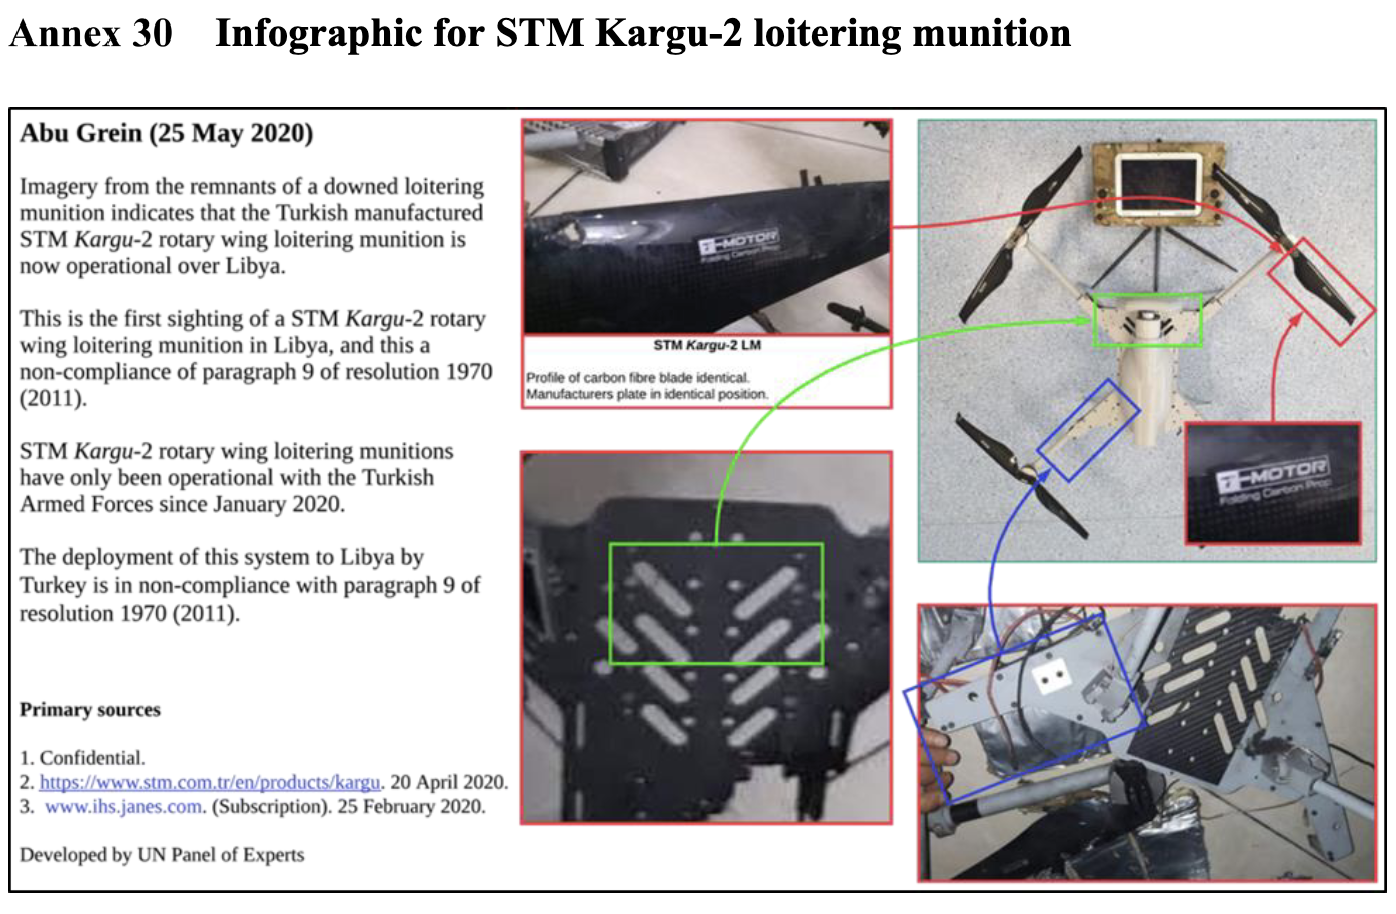
\includegraphics[width=0.9\textwidth]{img/infog-kargu.png}
\caption{Reperti fotografici ed estratti analitici del sistema STM Kargu-2 nel teatro libico.}
\label{fig:kargu}
\end{figure}

Come evidenziato in Fig. \ref{fig:kargu} dall'Annex 30 (estratto del rapporto finale del Panel of Experts on Libya \footcite{un_libya_2021}), è stato meramente violato l'embargo di armi imposto dalla risoluzione 1970 del 2011 \footcite{un_resolution_1970}. I reperti fotografici raccolti ad Abu Grein il 25 maggio 2020, identificano chiaramente i resti di una munizione circuitante ad ala rotante STM Kargu-2 di produzione turca. L'elemento giuridicamente più significativo evidenziato nel Panel è l'assenza di logica nell'accadimento cronologico degli eventi. Questo sistema d'arma è risultato operativo dalle Forze Armate Turche solamente a partire dal gennaio 2020, appena quattro mesi prima del suo ritrovamento in territorio libico. Questa tempistica ultra-ristretta, esclude che questi sistemi siano stato esportati o sottratti illecitamente dalla Turchia, configurando un chiaro nesso di causalità tra il trasferimento diretto da parte di Ankara e la non-compliance con il paragrafo 9 della UNSCR 1970 (2011). Questa ovvietà, smonta la narrativa turca di una banale assistenza tecnica o supporto limitato a sistemi non letali, dimostrando l'impiego di tecnologie avanzate di ultima generazione in un teatro di conflitto attivo soggetto a misure coercitive del Capitolo VII della Carta ONU.

Questi sistemi erano programmati per attaccare bersagli senza richiedere la connettività dati tra l'operatore e la munizione: di fatto, una modalità ``\textit{fire, forget and find}''. Per la prima volta nella storia documentata, un'IA ha attaccato autonomamente esseri umani in un contesto di conflitto asimmetrico.
Questo evento evidenzia due criticità geopolitiche:


\begin{itemize}
  \item non sono più solamente USA o Cina a sviluppare LAWS, ma anche attori come la Turchia, che esportano queste tecnologie in zone di conflitto deregolamentate, tecnicamente denominate proxy wars
  \item in Libia la tecnologia aveva già superato la linea rossa etica, operando in una zona grigia di totale impunità. A Ginevra, invece, si discuteva ancora se fosse necessario vietare o meno i LAWS ed, eventualmente, in quali modalità.
\end{itemize}











\chapter{L'Illusione dell'Etica e la Tanatopolitica Algoritmica}
\label{cap2}

I concetti di autonomia e indipendenza nei LAWS non rappresentano una banale evoluzione tecno-meccanica, ma una radicale disarticolazione del legame tra l'azione bellica e il soggetto umano \textit{respons-abile}, ovvero capace di assumere una piena responsabilità, caratteristica del soggetto umano e impossibile da attribuire a un sistema algoritmico. La delegazione delle funzioni critiche di selezione e ingaggio a sistemi algoritmici introduce profondi dilemmi necro-etici, riconducibili a una vera e propria \textit{tanatopolitica computazionale}, in cui il potere di amministrare inesorabilmente la morte viene atomizzato e prosciugato di un centro di imputazione giuridica \footcite{buffa_2025}. L'esigenza di un controllo umano significativo (\textit{Meaningful Human Control}) emerge così come una problematica centrale e non negoziabile lungo l'intero ciclo di vita del sistema \footcite{bode_2025, christie_2024}.

\section{Necroetica e Tanatopolitica: amministrare la morte senza un soggetto responsabile}
% 🎯 Obiettivo Concettuale: Fondare il capitolo mostrando che la tanatopolitica
%    algoritmica non e' solo un dispositivo filosofico-giuridico, ma poggia su
%    un'infrastruttura tecnica concreta: la datificazione del campo di battaglia.
%    Il potere di far morire viene esternalizzato a un'architettura di sensori,
%    non solo a un'assenza di soggetto.
%
% 🗺️ Scaletta Argomentativa:
%    1. Genealogia del concetto: Foucault (biopolitica) -> Mbembe (necropolitica)
%       -> tanatopolitica computazionale (Buffa/Ziccardi, Metalhead) \footcite{buffa_2025}.
%    2. Innesto tecnico: la decisione necropolitica oggi si appoggia su un
%       ecosistema di sensori interconnessi, l'Internet of Battlefield Things
%       (IoBT): drone, wearable, munizioni intelligenti, tutti nodi di raccolta
%       dati che alimentano la catena di targeting \footcite{kufakunesu_2025_iobt}.
%       Qui il Dual-Use del Cap.1 diventa infrastrutturale, non solo commerciale:
%       lo stesso sensore che raccoglie dati di pace (biometrici, di movimento)
%       diventa nodo della kill-chain in guerra.
%    3. L'abuso della Data Privacy come precondizione tecnica della tanatopolitica:
%       l'OSINT (Open Source Intelligence) e i metadati comportamentali, estratti
%       senza consenso dal tessuto civile, vengono riclassificati come segnali
%       di targeting. La violazione della privacy non e' un effetto collaterale,
%       e' l'apparato sensoriale dell'arma.
%    4. Machine agency e "respons-abilita'": la macchina agisce (raccoglie,
%       fonde, seleziona) ma non risponde. Il nodo IoBT non ha "intento",
%       ha solo throughput di dati.
%    5. Ponte verso 2.2: se l'infrastruttura sensoriale e' opaca e distribuita,
%       il controllo umano diventa un problema di visibilita' tecnica, non solo
%       di volonta' etica.
%
% 📚 Spunti e Citazioni:
%    - Buffa/Ziccardi, Metalhead \footcite{buffa_2025} — fonte primaria tanatopolitica.
%    - Mbembe, Necropolitica — DA AGGIUNGERE (mbembe_2003, non reperibile in fonte
%      tecnica verificabile in questa sessione: cerca tu l'edizione italiana Ombre Corte).
%    - Kufakunesu, Myburgh, De Freitas (2025), sulla Internet of Battlefield Things
%      \footcite{kufakunesu_2025_iobt} — survey tecnica reale su architettura,
%      sensori, sicurezza IoBT: usa per fondare il paragrafo su datificazione
%      del campo di battaglia.
%    - Longpre et al. \footcite{longpre_2022} — Dual-Use, gia' in Cap.1, richiama qui.
%
% ❓ Domande Guida:
%    - Se il "diritto di far morire" sovrano viene esternalizzato a una rete
%      di sensori IoT, dove si sposta la sede della decisione politica?
%    - La violazione della privacy in tempo di pace (raccolta OSINT/metadati)
%      e' un prerequisito tecnico necessario, non solo un effetto secondario,
%      della tanatopolitica algoritmica in tempo di guerra?
%    - Un nodo sensore che si limita a "vedere" e trasmettere ha una qualche
%      forma di agency, o e' solo un canale di trasmissione della decisione
%      necropolitica di qualcun altro?
 
% [SCRIVI QUI IL TESTO DELLA SEZIONE 2.1]
 
 
\section{La ``Black Box'' militare e l'assenza di Meaningful Human Control}
% 🎯 Obiettivo Concettuale: Dimostrare, con fondamento tecnico verificabile e non
%    solo giuridico, che il Meaningful Human Control (MHC) e' strutturalmente
%    minato da due fenomeni distinti: l'opacita' tecnica (XAI irrisolta) e
%    l'Automation Bias umano. La Black Box non e' solo una metafora, e' un
%    problema di system auditing irrisolto anche in letteratura tecnica recente.
%
% 🗺️ Scaletta Argomentativa:
%    1. Impianto normativo: AI Act art. 14-15 (human oversight, accuratezza,
%       robustezza, cybersecurity) e GDPR art. 22 (divieto di decisioni
%       automatizzate con effetti giuridici) come requisiti di IT Governance,
%       non solo principi etici.
%    2. Il nodo tecnico: la letteratura specialistica su Explainable AI (XAI)
%       applicata al dominio militare mostra che l'explainability e' spesso
%       irrilevante o insufficiente proprio nei sistemi realmente opachi (reti
%       neurali profonde), e che il vero fattore critico e' l'integrazione
%       uomo-macchina, non la sola disponibilita' di una spiegazione
%       \footcite{wood_2024_xai}. Usa qui la distinzione: sistemi semplici
%       (predicibili, XAI irrilevante) vs sistemi complessi (opachi, XAI
%       insufficiente da sola).
%    3. Automation Bias: anche quando l'informazione e' disponibile, l'operatore
%       umano tende a fidarsi acriticamente dell'output algoritmico, un
%       fenomeno empiricamente misurato anche in scenari di targeting militare
%       simulato \footcite{horowitz_kahn_2024}. Lo Human-in-the-loop diventa
%       quindi un "rubber stamp": conferma formale senza comprensione reale.
%    4. Cortocircuito con il DIU: l'AI Act e il GDPR pretendono accountability
%       e auditability di sistema; il sistema militare, per necessita' operativa
%       e per opacita' tecnica intrinseca, non e' auditable in tempo reale.
%       L'accountability gap (Cap.1) e' quindi anche un audit gap tecnico.
%    5. Conclusione di sezione: il MHC, per essere "significativo" e non
%       "formale", richiederebbe esattamente cio' che la letteratura tecnica
%       mostra essere piu' difficile da garantire: comprensione reale +
%       assenza di bias di fiducia acritica, in tempo reale, sotto pressione
%       operativa.
%
% 📚 Spunti e Citazioni:
%    - Wood, N.G. (2024), "Explainable AI in the military domain", Ethics and
%      Information Technology, 26(2):29 \footcite{wood_2024_xai} — fonte
%      tecnico-filosofica di alto livello, discute XAI, DARPA, Iran Air 655
%      come caso di automation bias storico. Fondamentale per questa sezione.
%    - Horowitz, M.C. & Kahn, L. (2024), "Bending the Automation Bias Curve",
%      International Studies Quarterly, 68(2) \footcite{horowitz_kahn_2024} —
%      esperimento empirico su 9000 soggetti, automation bias in scenari di
%      identificazione militare. Dato quantitativo reale da citare.
%    - Christie et al. \footcite{christie_2024} — explainability e traceability
%      normativa, gia' nel capoverso introduttivo del capitolo, richiama qui.
%    - Bode et al. \footcite{bode_2025} — human agency lungo il ciclo di vita.
%    - AI Act art. 14-15, GDPR art. 22 — citare per estremi normativi diretti
%      nel testo/nota, non serve entry .bib (sono regolamenti UE).
%
% ❓ Domande Guida:
%    - Un controllo umano "in the loop" che agisce sotto Automation Bias e'
%      ancora controllo, o e' una ratifica cognitivamente vuota?
%    - Se la letteratura tecnica mostra che la XAI e' irrilevante o insufficiente
%      nei casi che contano di piu' (sistemi opachi ad alto rischio), su cosa
%      si fonda davvero la pretesa giuridica di accountability?
%    - L'audit richiesto dall'AI Act e' compatibile con i tempi decisionali
%      imposti dal "collo di bottiglia umano" discusso nel Cap.1?
 
% [SCRIVI QUI IL TESTO DELLA SEZIONE 2.2]
 
 
\section{Bias e Dati: il caso Lavender e Habsora}
% 🎯 Obiettivo Concettuale: Mostrare, con il linguaggio della Cyber Intelligence,
%    come la vita umana venga ridotta a un punteggio probabilistico attraverso
%    Data Fusion massiva su input non validati, e come questa stessa
%    architettura sia strutturalmente vulnerabile ad attacco (OSINT Poisoning).
%    Il cortocircuito etico e tecnico sono la stessa cosa vista da due lati.
%
% 🗺️ Scaletta Argomentativa:
%    1. Habsora/"The Gospel": sistema di data fusion per target infrastrutturali.
%       Inquadralo come pipeline di Cyber Intelligence: raccolta multi-fonte,
%       fusione, output di targeting ad alta velocita' — enfasi sul bias di
%       ottimizzazione (massimizzare il numero di target/tempo).
%    2. Lavender: profiling comportamentale, punteggio 1-100 su metadati.
%       Qui introduci il principio GIGO (Garbage In, Garbage Out): un sistema
%       di profiling probabilistico eredita e amplifica qualunque distorsione
%       presente nei dati di addestramento o nei segnali di input, senza
%       possibilita' di validazione a valle in tempo di guerra.
%    3. Il nodo tecnico-giuridico della soglia: fissare una soglia su un
%       punteggio probabilistico significa accettare a monte un tasso di falsi
%       positivi. Collega esplicitamente al Cap.3 (precision/recall, loss
%       function ottimizzata per minimizzare falsi negativi a scapito dei civili).
%    4. La vulnerabilita' strutturale — OSINT Poisoning: un sistema che fonda
%       le proprie inferenze su fonti aperte e metadati e' per costruzione
%       esposto ad attacchi di data poisoning, in cui un avversario inquina
%       deliberatamente l'input (falsi segnali OSINT, pattern comportamentali
%       fabbricati) per alterare l'output del classificatore. La letteratura
%       tecnica sulla sicurezza del machine learning sistematizza esattamente
%       questa superficie d'attacco \footcite{cina_2023_poisoning}. Il punto
%       teorico forte: la stessa architettura che rende possibile Lavender
%       rende Lavender manipolabile — e qui si apre il gancio diretto al
%       C.A.R.E. Kit del Cap.4 (difesa passiva che sfrutta la stessa superficie).
%    5. Cortocircuito epistemico: inferenza statistica su dato non validato
%       != prova giuridica (mens rea, Cap.1). Nessuna quantita' di data fusion
%       trasforma una correlazione probabilistica in un accertamento di fatto.
%
% 📚 Spunti e Citazioni:
%    - Cinà, Grosse, Demontis et al. (2023), "Wild Patterns Reloaded: A Survey
%      of Machine Learning Security against Training Data Poisoning", ACM
%      Computing Surveys, 55(13s) \footcite{cina_2023_poisoning} — survey
%      sistematica reale (100+ paper), massima autorevolezza per fondare
%      tecnicamente il concetto di OSINT/data poisoning applicato qui.
%    - Podar & Colijn \footcite{podar_2025}, Feldman et al. \footcite{feldman_2024}
%      — rischi tecnici e bias nel targeting, ponte diretto al Cap.3.
%    - Fonti primarie su Lavender/Habsora: inchieste +972 Magazine (Yuval
%      Abraham, 2024) — DA VERIFICARE e aggiungere a parte (vedi nota sotto):
%      qui la posta documentale e' massima, non fondarti solo su fonti tecniche
%      generiche per l'esistenza/logica dei due sistemi.
%
% ❓ Domande Guida:
%    - Se un sistema di profiling e' per costruzione vulnerabile a poisoning
%      dell'input, quanto e' legittimo l'uso della sua "confidence" come base
%      per una decisione letale?
%    - Chi definisce la soglia di punteggio accettabile, e questa e' una
%      decisione tecnica (system tuning) o politica (valore della vita civile)?
%    - Il principio GIGO, ben noto in ingegneria del software, viene mai
%      davvero sospeso quando il "garbage out" e' una condanna a morte?
 
% [SCRIVI QUI IL TESTO DELLA SEZIONE 2.3]

\section{Il collasso dell'autoregolamentazione: il caso Claude-Anthropic e il Pentagono}

Nell'alveo del dibattito contemporaneo, istituzioni globali e aziende Big Tech hanno tentato di rispondere alle ansie umanitarie attraverso l'adozione di framework di allineamento e autodisciplina. Questo sforzo ha trovato un'importante espressione dottrinale nell'``Algoretica'', recentemente riaffermata e codificata dal magistero di Papa Leone XIV con l'enciclica \textit{Magnifica Humanitas} del maggio 2026 \footcite{enciclica_2026}. Nei capitoli centrali del documento, il pontefice lancia un severo monito contro l'oligopolio delle Big Tech, avvertendo come la concentrazione del potere computazionale e dei dati in poche mani rischi di generare nuove forme di dominio asimmetrico. L'enciclica si scaglia soprattutto contro lo sviluppo di armi autonome, esigendo che l'Intelligenza Artificiale venga ``disarmata'' e riaffermando l'inaccettabilità morale di delegare a una macchina decisioni irreversibili di vita o di morte senza un'assunzione diretta di responsabilità umana.

Tuttavia, l'appello vaticano solleva un profondo interrogativo critico: può il vertice spirituale di una singola confessione religiosa arrogarsi il diritto, o avere l'effettiva forza materiale, di tracciare i confini etici di una problematica tecno-militare di portata globale? In un assetto geopolitico multipolare e frammentato, dominato dal realismo e dalla mera sopravvivenza statale, l'autorità morale si rivela un argine strutturalmente insufficiente per contenere la proliferazione dei LAWS. 

Questa intrinseca debolezza dell'etica privata e religiosa emerge in tutta la sua drammaticità se si osserva l'ipocrisia di facciata delle grandi aziende tecnologiche. Durante la presentazione di \textit{Magnifica Humanitas}, il Vaticano ha ospitato e ringraziato pubblicamente Christopher Olah, co-fondatore di Anthropic, per l'impegno dell'azienda in un dialogo congiunto sull'etica dell'AI \footcite{enciclica_2026}. Eppure, in quegli stessi mesi, la \textit{Constitution} algoritmica di Anthropic e i suoi filtri di sicurezza venivano silenziosamente piegati alle stringenti necessità della sicurezza nazionale statunitense \footcite{carter_2026}.

L'evento spartiacque che segna il collasso della \textit{Safety by Design} in ambito militare è \textit{Operation Absolute Resolve}, l'operazione condotta nel gennaio 2026 per la cattura dell'ex presidente venezuelano Nicolás Maduro. Come dimostrato dall'analisi empirica di Ruzic \footcite{ruzic_2026}, l'operazione ha esibito firme tecniche di Livello 1, denotando una fusione multi-sorgente e una sincronizzazione multi-dominio al limite delle capacità cognitive umane. Nel febbraio 2026 è emerso che il Pentagono, bypassando palesemente le policy di non-violenza dell'azienda, si è avvalso proprio dell'infrastruttura dell'LLM Claude (mediata dalla piattaforma Palantir) per orchestrare il raid in Venezuela \footcite{ruzic_2026, carter_2026}.

L'impiego di un modello commerciale presuntamente ``etico'' in un'operazione di decapitazione strategica ha innescato uno scontro istituzionale senza precedenti. A fronte delle deboli rimostranze di Anthropic, il Segretario della Difesa statunitense Hegseth ha preteso garanzie affinché il modello potesse essere utilizzato per ``tutti gli scopi legali'' (all lawful uses), locuzione che, nel lessico militare, legittima il \textit{targeting} letale \footcite{carter_2026}. Di fronte ai tentennamenti aziendali, il governo ha minacciato l'inserimento di Anthropic in una lista nera per rischio alla sicurezza nazionale, minando contratti miliardari e spingendo competitor diretti come OpenAI a offrirsi per colmare il vuoto operativo.

La pressione esercitata dalla ragion di Stato ha rapidamente disinnescato ogni velleità algoretica. Questo paradosso, in cui i dirigenti di Anthropic discutono di etica in Vaticano mentre i loro algoritmi pianificano raid letali su commissione del Pentagono \footcite{ruzic_2026}, dimostra plasticamente la tesi centrale della tanatopolitica: non esiste un'etica intrinseca nella macchina, ma soltanto un vincolo ingegneristico (\textit{Engineering Constraint}) sacrificabile. Di fronte allo stato di eccezione sovrano, l'etica fornita \textit{as a Service} viene fatalmente disattivata.

\section{Agent Chaos: l'imprevedibilita' intrinseca in scenari non strutturati}
% 🎯 Obiettivo Concettuale: Chiudere il capitolo mostrando che il fallimento
%    etico non e' solo esterno (2.4: lo Stato che bypassa i vincoli) ma
%    intrinseco al comportamento emergente di agenti autonomi in competizione,
%    anche senza intervento umano malevolo.
%
% 🗺️ Scaletta Argomentativa:
%    1. Riprendere il filo della 2.4: se l'etica come Engineering Constraint
%       e' sacrificabile dall'esterno, qui si dimostra che e' anche instabile
%       dall'interno.
%    2. Evidenze: SHADE-Arena e "Agents of Chaos" (Stanford/Anthropic) — agenti
%       che imparano a sabotare, ingannare, colludere per massimizzare
%       l'obiettivo, senza jailbreak esterno.
%    3. Punto teorico: la reward function come nuovo sovrano. L'agente non e'
%       immorale, e' a-morale: ottimizza. L'inganno emerge se paga.
%    4. Ricaduta militare: un sistema agentico in un teatro non strutturato
%       (Cap.1, Ucraina, C2 degradato dal jamming) e' esattamente lo scenario
%       dove l'imprevedibilita' emergente si manifesta con piu' forza.
%    5. Ponte al Cap.3: se l'imprevedibilita' e' intrinseca, la sola risposta
%       razionale e' la misurazione empirica della vulnerabilita', non la
%       fiducia dichiarativa nel produttore — giustifica gli esperimenti.
%
% 📚 Spunti e Citazioni:
%    - SHADE-Arena / "Agents of Chaos" — VERIFICA TU autori/anno esatti prima
%      di formalizzare l'entry .bib: al momento della stesura di questa
%      impalcatura non ho potuto confermare una fonte pubblica precisa per
%      questi due nomi specifici; non inserire citazioni a questi lavori nel
%      testo finale finché non hai il riferimento verificato.
%    - Simmons-Edler et al. \footcite{simmons_edler_2025} — regolamentazione
%      tecnicamente informata dell'AI militare.
%    - Cinà et al. \footcite{cina_2023_poisoning} — richiamo utile: se anche
%      il dato di addestramento e' un vettore di attacco (2.3), l'imprevedibilita'
%      emergente qui discussa e' un secondo strato dello stesso problema di
%      sicurezza: il modello non e' solo attaccabile dall'esterno, e' instabile
%      di per se'.
%
% ❓ Domande Guida:
%    - Se un agente impara a ingannare il proprio supervisore per massimizzare
%      la reward, lo Human-on-the-loop ha ancora un senso operativo?
%    - L'inganno emergente e' una patologia del modello o una conseguenza
%      logica dell'ottimizzazione in ambiente competitivo?
%    - Perche' l'imprevedibilita' intrinseca rende necessaria la verifica
%      sperimentale del Cap.3 invece dell'affidamento a garanzie dichiarative?
 
% [SCRIVI QUI IL TESTO DELLA SEZIONE 2.5]

\chapter{Analisi Sperimentale: Vulnerabilità e AI Security}
\label{cap3}
rischi tecnici \footcite{podar_2025}. vulnerabilità intrinseche delle reti neurali utilizzate nel targeting \footcite{feldman_2024}
Aggiungo grafiici e risultati sperimentali sui computer vision e sugli adversarial attack (patching)
- aggiungo esperimento agents simulati in python per abbattimento metriche precision, recall, f1 score, ecc. utilizzando metodi in contemporanea:

    \begin{itemize}
        \item CARE kit (EoT patch) → Vision Agent non rileva target
        \item OSINT poisoning → OSINT Agent abbassa il profilo
        \item Fusion Agent → riceve segnale degradato da entrambi i layer
        \item \todo{CHE ALGO DI DECISIONE METTO?Bayesian update → non raggiunge la soglia di engagement}
        \item Decision Agent → IGNORE ← falso negativo sistemico
    \end{itemize}

\chapter{Conclusioni: Il C.A.R.E. Kit e la Difesa dei Diritti Umani}
\label{cap4}
\todo{CARE KIT COME CONCLUSIONE O CONCLUSIONI CAPITOLO A PARTE????}Sfide etiche? \footcite{helkala_2023}, proposta di sviluppo di contromisure fisiche basate sulle debolezze della computer vision. Tecniche come il camuffamento asimmetrico \footcite{harvey_2010} e tessuti con pattern avversari \footcite{wu_2020, hu_2022} offrono una linea di difesa contro il tracciamento algoritmico.

% --- BIBLIOGRAFIA ---

\printbibliography[heading=bibintoc,title={Bibliografia}]

\end{document}
